\documentclass{bmstu}

\bibliography{biblio}

\begin{document}

\makecourseworktitle{Информатика и системы управления}{Программное обеспечение ЭВМ и информационные технологии}{Визуализация дисперсии света на прозрачных предметах}{ИУ7-53Б}{Д.~В.~Недолужко}{Н.~В.~Новик}{}{}

\maketableofcontents

% \begin{definitions}
	\definition{}{}
\end{definitions}
% \begin{abbreviations}
	\definition{}{}
\end{abbreviations}

\chapter*{ВВЕДЕНИЕ}
\addcontentsline{toc}{chapter}{ВВЕДЕНИЕ}

    Дисперсия - это разбиения белого пучка света на его цветные составляющие при прохождении через прозрачные поверхности. Наиболее известным экспериментом, показывающим это явление, является пропускание белого пучка света через призму и наблюдение светового спектра на экране. Явление дисперсии также иллюстрируют радуга и блеск драгоценных камней.

    Явление дисперсии занимало ума людей столетиями. Инженеры, проектирующие оптические приборы, стремились минимизировать ее проявление в своих приборах. В то время как ювелиры находились в постоянном стремлении преумножить блеск своих драгоценных камней.

    Дисперсия повсюду встречается в нашей жизни, это явление подробно изучено с физической точки зрения. При построении изображений, претендующих на фотореалистичность, нельзя не учитывать это явление.

    % TODO: изменить вывод в соответствии с новыми целью и задачами

    Целью моего проекта является разработка программного обеспечения для визуализации трехмерных объектов и наблюдения дисперсии света на прозрачных поверхностях c возможностью выбора пользователем объектов сцены из предложенного списка, а также задания источников освещения по их характеристикам: положению, интенсивности.

    Для достижения поставленной цели необходимо решить следующие задачи:

    \begin{itemize}
        \item изучение явления дисперсии с физической точки зрения;
        \item анализ существующих алгоритмов построения реалистичных изображений;
        \item выбор алгоритма для решения поставленной задачи;
        \item проектирование архитектуры и графического интерфейса программы;
        \item реализация структур данных и алгоритмов;
	    \item описание структуры разрабатываемого ПО;
	    \item написание программы;
        \item исследование производительности программы.
    \end{itemize}

\chapter{Аналитический раздел}

    В данном разделе рассматриваются существующие алгоритмы построения реалистичных изображений. Так же, обосновывается выбор реализуемого алгоритма и указывается список ограничений, в рамках которых будет работать разрабатываемое ПО.
    
    \section{Описание алгоритмов удаления невидимых линий и поверхностей}

        \subsection {Некоторые теоретические сведения}
        
            Прежде чем описывать алгоритмы, нужно дать некоторые определения, которые будут использованы в данном разделе.
            
            Алгоритмы удаления невидимых линий и поверхностей служат для определения линий ребер, поверхностей, которые видимы или невидимы для наблюдателя, находящегося в заданной точке пространства \cite{rogers}.
            
            Решать задачу можно в:
            \begin{itemize}
            	\item объектном пространстве - мировая системе координат, высокая точность. Обобщенный подход, основанный на анализе пространства объектов, предполагает попарное сравнение положения всех объектов по отношению к наблюдателю.
            	\item пространстве изображений - в экранных координатах, системе координат, связанной с тем устройством в котором отображается результат. (Графический дисплей).
            \end{itemize}
            
            Под экранированием подразумевается загораживание одного объекта другим.
            
            Под глубиной подразумевается значение координаты Z, направленной от зрителя, за плоскость экрана.
        
        \subsection{Алгоритм Робертса}
        
            Алгоритм Робертса решает задачу удаления невидимых линий. Работает в объектном пространстве. Данный алгоритм работает исключительно с выпуклыми телами. Если тело изначально является не выпуклым, то нужно его разбить на выпуклые составляющие. Алгоритм целиком основан на математических предпосылках \cite{rogers}.

            Из-за сложности математических вычислений, используемых в данном алгоритме, а так же из-за дополнительных затраты ресурсов на вычисление матриц данный алгоритм является довольно медленным.
        
        \subsection{Алгоритм Варнака}
        
            Алгоритм Варнака \cite{rogers,shykin,bayackovskiy} позволяет определить, какие грани или части граней объектов сцены видимы, а какие заслонены гранями других объектов. Так же как и в алгоритме Робертса анализ видимости происходит в пространстве изображения. В качестве граней обычно выступают выпуклые многоугольники, алгоритмы работы с ними эффективнее, чем с произвольными многоугольниками. Окно, в котором необходимо отобразить сцену, должно быть прямоугольным. Алгоритм работает рекурсивно, на каждом шаге анализируется видимость граней и, если нельзя легко определить видимость, окно делится на 4 части и анализ повторяется отдельно для каждой из частей (см. рис. \ref{img:Warnock_1}).
            
            \imgs{Warnock_1}{ht!}{0.7}{Пример разбиения Алгоритмом Варнока}
            
                Так как данный алгоритм основывается на рекурсивном разбиении экрана, в зависимости от расположения объектов это может вызвать, как положительной, так и отрицательный эффект. Чем меньше пересечений объектов, тем быстрее алгоритм завершит свою работу.
        
        \subsection{Алгоритм Z--буфера}
        
            Алгоритм Z--буфера \cite{rogers,shykin} позволяет определить, какие пикселы граней сцены видимы, а какие заслонены гранями других объектов. Z--буфер -– это двухмерный массив, его размеры равны размерам окна, таким образом, каждому пикселу окна, соответствует ячейка Z-буфера. В этой ячейке хранится значение глубины пиксела (см. рис. \ref{img:z-buff}). Перед растеризацией сцены Z--буфер заполняется значением, соответствующим максимальной глубине. В случае, когда глубина характеризуется значением w, максимальной глубине соответствует нулевое значение. Анализ видимости происходит при растеризации граней, для каждого пиксела рассчитывается глубина и сравнивается со значением в Z--буфере, если рисуемый пиксел ближе (его \texttt{w} больше значения в Z--буфере), то пиксел рисуется, а значение в Z--буфере заменяется его глубиной. Если пиксел дальше, то пиксел не рисуется и Z--буфер не изменяется, текущий пиксел дальше того, что нарисован ранее, а значит невидим. 
            
            \imgs{z-buff}{h!}{0.7}{Пример работы алгоритма Z--буфера}
            
            К недостаткам алгоритма следует отнести довольно большие объемы требуемой памяти, а также имеются другие недостатки, которые состоят в трудоемкости устранения лестничного эффекта и трудности реализации эффектов прозрачности.
        
        \subsection{Алгоритм прямой трассировки лучей}
        
            Основная идея алгоритма прямой трассировки лучей \cite{shykin} состоит в том, что наблюдатель видит объекты благодаря световым лучам, испускаемым некоторым источником, которые падают на объект, отражаются, преломляются или проходят сквозь него и в результате достигают зрителя.
            
            Основным недостатком алгоритма является излишне большое число рассматриваемых лучей, приводящее к существенным затратам вычислительных мощностей, так как лишь малая часть лучей достигает точки наблюдения. Данный алгоритм подходит для генерации статических сцен и моделирования зеркального отражения, а так же других оптических эффектов \cite{traceproblem}.
        
        \subsection{Алгоритм обратной трассировки лучей}
        
            Алгоритм обратной трассировки лучей отслеживает лучи в обратном направлении (от наблюдателя к объекту) \cite{shykin}. Такой подход призван повысить эффективность алгоритма в сравнении с алгоритмом прямой трассировки лучей. Обратная трассировка позволяет работать с несколькими источниками света, передавать множество разных оптических явлений \cite{snizko}.
            
            Пример работы данного алгоритма приведен на рисунке \ref{img:trace_scheme}.
            
            \imgs{trace_scheme}{h!}{0.7}{Пример работы алгоритма обратной трассировки лучей}
            
            Считается, что наблюдатель расположен на положительной полуоси z в бесконечности, поэтому все световые лучи параллельны оси z. В ходе работы испускаются лучи от наблюдателя и ищутся пересечения луча и всех объектов сцены \cite{bayackovskiy}. В результате пересечение с максимальным значением z является видимой частью поверхности и атрибуты данного объекта используются для определения характеристик пикселя, через центр которого проходит данный световой луч. 
            
            Для расчета эффектов освещения сцены проводятся вторичные лучи от точек пересечения ко всем источникам света. Если на пути этих лучей встречается непрозрачное тело, значит, данная точка находится в тени.
            
            Несмотря на более высокую эффективность алгоритма в сравнении с прямой трассировкой лучей, данный алгоритм считается достаточно медленным, так как в нем происходит точный расчет сложных аналитических выражений для нахождения пересечения с рассматриваемыми объектами.
        
    \section{Описание алгоритмов построения теней}
        
        Для создания реалистичного изображения в компьютерной графике применяются различные алгоритмы освещения.
        
        Модель освещения предназначена для расчета интенсивности отраженного к наблюдателю света в каждой точке изображения.
        
        Модель освещения может быть:
        \begin{itemize}
            \item локальной - в данной модели учитывается только свет от источников и ориентация поверхности.
            \item глобальной - в данной модели, помимо составляющих локальной, учитывается еще и свет, отраженный от других поверхностей или пропущенный через них.
        \end{itemize}
        
        Локальная модель включает 3 составляющих:
        \begin{enumerate}
        	\item Диффузную составляющую отражения.
        	\item Отражающую составляющую отражения.
        	\item Рассеянное освещение.
        \end{enumerate}
        
        Выбор алгоритма построения теней напрямую зависит от выбора алгоритма отсечения невидимых ребер и поверхностей, а так же - от выбора модели освещения. 
        
        Так в алгоритме трассировки лучей тени получаются практически без дополнительных вычислений, а в алгоритме с Z буфером, к примеру, можно получить тени, используя второй буфер, полученный подменой точки наблюдения на точку источника света. 
        
    \section{Вывод}
        
        Оценив все изложенные выше алгоритмы, можно сделать вывод, что для данной работы лучше всего подходит алгоритм обратной трассировки лучей, так как он точно отражает суть физических явлений, таких как отражение и преломление лучей.

\chapter{Конструкторский раздел}

    В данном разделе будут рассмотрены требования к программному обеспечению, а также схемы алгоритмов, выбранных для решения поставленной задачи. Так же, будут описаны пользовательские структуры данных и приведена структура реализуемого программного обеспечения.
    
    \section{Разработка алгоритмов}
    
        \subsection{Основные физические соотношения для дисперсии}
    
            Дисперсия света обусловлена зависимостью показателей преломления света от длины волны. Закон Снеллиуса (также Снелля или Снелла) описывает преломление света на границе двух прозрачных сред.
        
            Угол падения света на поверхность связан с углом преломления соотношением \eqref{eq:dis}:
        
            \begin{equation}
               n_{1} sin(\theta_{1}) = n_{2} sin(\theta_{2}) \label{eq:dis}
            \end{equation}
            
            где $n_{1}$ — показатель преломления среды, из которой свет падает на границу раздела;
            
            $\theta_{1}$ — угол падения света — угол между падающим на поверхность лучом и нормалью к поверхности;
            
            $n_{2}$ — показатель преломления среды, в которую свет попадает, пройдя границу раздела;
            
            $\theta_{2}$ — угол преломления света — угол между прошедшим через поверхность лучом и нормалью к поверхности.
            
    
            Формула Зельмейера \eqref{eq:zel} — это эмпирическая формула описывающая зависимость между показателем преломления и длиной волны для конкретной прозрачной среды. Уравнение используется для определения дисперсии света в этой среде. 
            
            \begin{equation}
                n^2(\lambda) = 1 + \sum_{i}^{} \frac{B_i \lambda^2}{\lambda^2 - C_i}  \label{eq:zel}
            \end{equation}
            
            где \( n \) - показатель преломления;
            
            \( \lambda \) - длина волны;
            
            \( B_i, C_i \) - экспериментально определяемые коэффициенты Селлмейера.
    
        \subsection{Пересечение луча и сферы}
        
            Уравнение луча представлено ниже:

            \begin{equation}
            	P = O + t\overrightarrow{D}, t \geq 0,
            	\label{eq:ref5}
            \end{equation}
            где \( P \) -- точка лежащая на луче, \( O \) -- начало луча, $\overrightarrow{D}$ -- направление луча, \( t \) -- произвольное положительное действительное число.
            
            Сфера — это множество точек $P$, лежащих на постоянном расстоянии $r$ от фиксированной точки $C$. Тогда можно записать уравнение, удовлетворяющее этому условию:
            
            \begin{equation}
            	distance(P,C) = r
            	\label{eq:ref6}
            \end{equation}
            
            Запишем расстояние (\ref{eq:ref6}) между P и C как длину вектора из P в C.
            
            \begin{equation}
            	|P-C|=r
            \end{equation}
            
            Заменим на скалярное произведение вектора на себя:
            
            \begin{equation}
            	\sqrt{\langle P - C\rangle, \langle P - C\rangle} = r
            \end{equation}
            
            Избавимся от корня:
            
            \begin{equation}
            	\langle P - C\rangle, \langle P - C\rangle = r^2
            	\label{eq:ref7}
            \end{equation}
            
            В итоге есть два уравнения - уравнение луча и сферы. Найдем пересечение луча со сферой. Для этого подставим (\ref{eq:ref5}) в (\ref{eq:ref7})
            
            \begin{equation}
            	\langle O + t\overrightarrow{D} - C \rangle, \langle O + t\overrightarrow{D} - C\rangle = r^2
            \end{equation}
            
            Разложим скалярное произведение и преобразуем его. В результате получим:
            
            \begin{equation}
            	t^2 \langle \overrightarrow{D}, \overrightarrow{D} \rangle + 2t \langle \overrightarrow{OC}, \overrightarrow{D} \rangle + \langle \overrightarrow{OC}, \overrightarrow{OC} \rangle -r^2 = 0
            	\label{eq:ref8}
            \end{equation}
            
            Представленное квадратное уравнение (\ref{eq:ref8}) имеет несколько возможных случаев решения. Если у уравнения одно решение, то луч касается сферы. Два решения -- луч пересекает сферу. Нет решений -- луч не пересекается со сферой.

        \subsection{Описание алгоритма обратной трассировки}
        
            Суть алгоритма состоит в следующем: Из некоторой точки пространства, называемой виртуальным глазом, или камерой, через каждый пиксель изображения испускается луч и находится точка пересечения с объектом сцены. При обнаружении точки пересечения, формируется отраженный луч и испускается. Данный алгоритм повторяется рекурсивно, пока не достигнем максимальной установленной глубины рекурсии. Полученные цвета перемножаются.

            На рисунке \ref{fig:ray_tracing} представлена схема синтеза изображения с применением данного алгоритма.

            \begin{figure}
                \centering
                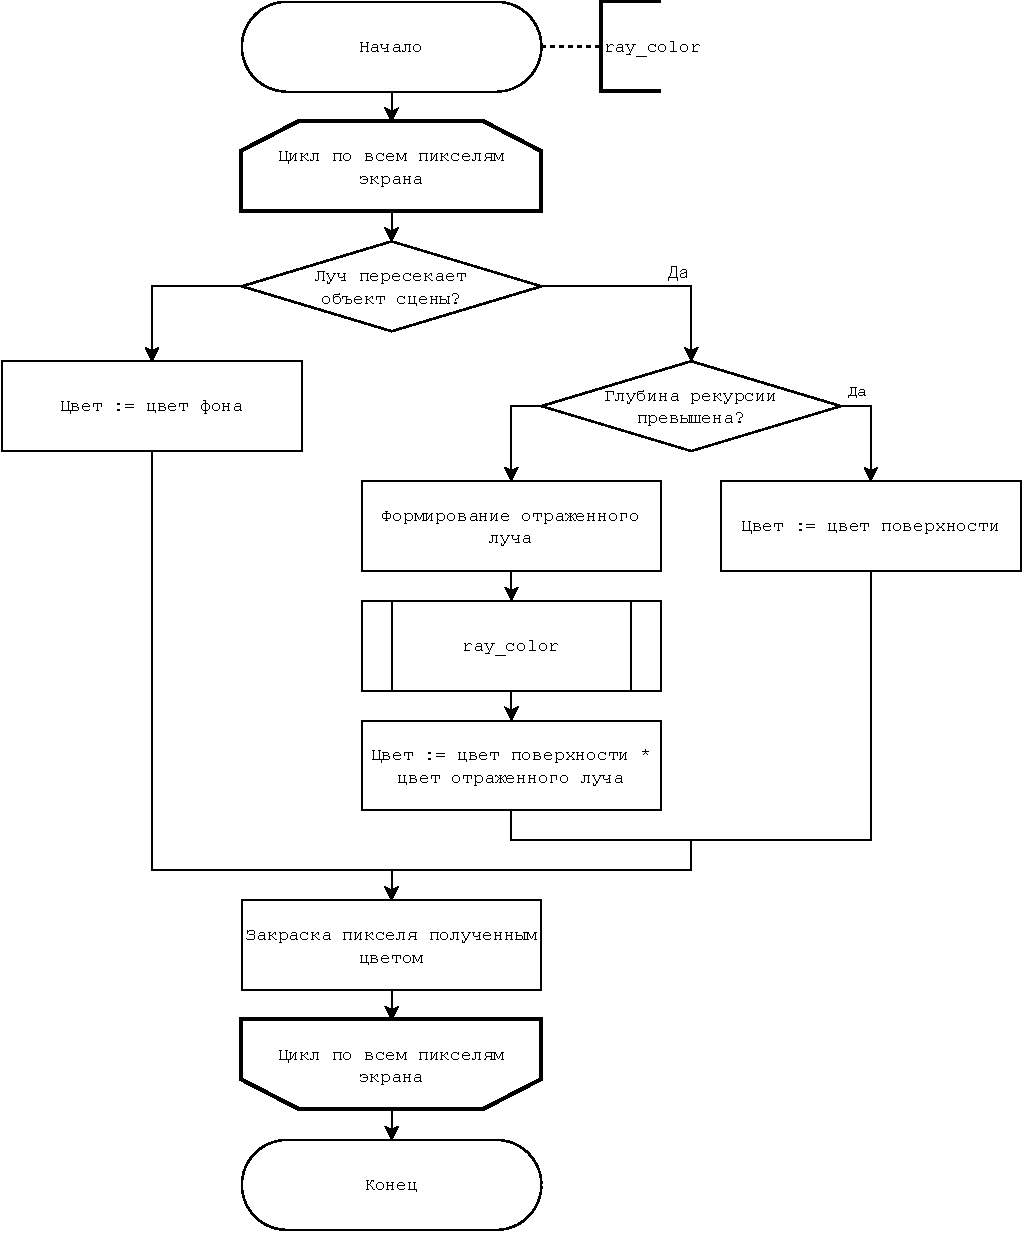
\includegraphics[width=\textwidth,height=25cm,keepaspectratio]{inc/img/ray_tracing.pdf}
                \caption{Схема алгоритма синтеза изображения с применением алгоритма обратной трассировки лучей} \label{fig:ray_tracing}
            \end{figure}

    \section{Описание используемых типов и структур данных}

        В данной работе используются следующие типы и структуры данных:
        
        \begin{itemize}
            \item источник света – задается расположением, направленностью и интенсивностью света;
            \item математические абстракции:
            \begin{itemize}
                \item точка -- хранит координаты x, y, z
                \item вектор -- хранит направление по x, y, z
            \end{itemize}
            \item цвет -- хранит три составляющие RGB модели цвета
        \end{itemize}

\clearpage

    \section{Описание структуры программного обеспечения}
    
            На рисунке \ref{fig:uml} представлена диаграмма классов реализуемого программного обеспечения. Объект класса \texttt{draw\_manager} генерирует изображение класса \texttt{image} для заданного положения камеры. Сцена состоит из объектов, удовлетворяющих интерфейсу \texttt{hittable}, который наследуют классы \texttt{sphere} и \texttt{hittable\_list}. Класс \texttt{hittable\_list} реализует паттер композит. Класс \texttt{sphere} агрегирует класс \texttt{material}, который в свою очередь алгегирует класс \texttt{texture}. Реализованы 4 типа материалов: матовый (\texttt{lambertian}), металлический (\texttt{metal}), прозрачный (\texttt{dieletric}), излучающий свет (\texttt{diffuse\_light}). И реализованы 2 типа текстур материалов: монотонный (\texttt{solid\_color}), клетчатый (\texttt{checker\_texture}).
        
        \begin{figure}
            \centering
            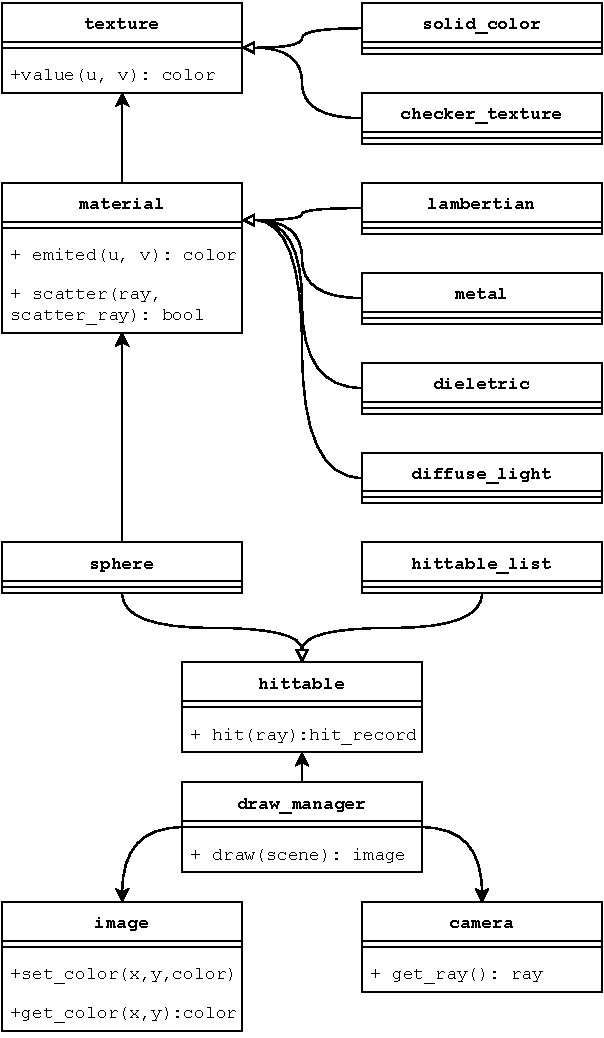
\includegraphics[width=\textwidth,height=25cm,keepaspectratio]{inc/img/uml.pdf}
            \caption{UML диаграмма разрабатываемого программного обеспечения}
            \label{fig:uml}
        \end{figure}

\clearpage

    \section{Вывод}

        В данном разделе были приведены основные физические соотношения для дисперсии, приведена схема алгоритма обратной трассировки лучей, описаны используемые структуры данных, приведена UML диаграмма разрабатываемого приложения.
\chapter{Технологический раздел}

    В данном разделе будут представлены средства разработки программного обеспечения, детали реализации и процесс сборки разрабатываемого программного обеспечения.
    
    \section{Выбор средств программной реализации}

        В качестве языка программирования для разработки программного обеспечения был выбран язык \texttt{C++} \cite{cpp}. Данный выбор обусловлен тем, что данный язык предоставляет весь функционал требуемый для решения поставленной задачи.

        Для создания пользовательского интерфейса ПО был использован фреймворк \texttt{QT} \cite{qt}. Данный фреймворк содержит в себе объекты, позволяющие напрямую работать с пикселями изображения, а  так же возможности создания интерактивных пользовательских интерфейсов, что позволит в интерактивном режиме управлять изображением.

        В качестве стиля кода был выбран стиль Mozilla \cite{fmtmozilla}. Для проведения автоформатирования был выбран инструмент \texttt{clang-format} \cite{clangfmt}, так как он поддерживает работу в командной строке, а так же реализован в качестве плагина для популярных ide.
        
        Для отслеживания утечек памяти был выбран инструмент \texttt{Valgrind} \cite{valgrind}.
        
        Для сборки программного обеспечения использовался инструмент \texttt{CMake} \cite{cmake}.
        
        В качестве среды разработки был выбран текстовый редактор \texttt{vim} \cite{vim}, поддерживающий работу в командной строке, а так же установкy плагинов \cite{vimawesome}, в том числе для работы с \texttt{C++} и \texttt{CMake}.

    \section{Процесс сборки приложения}

        Для сборки программного обеспечения использовался инструменты \texttt{CMake} \cite{cmake}.

        Для сборки приложения необходимо в командной строке, находясь в директории проекта, выполнить следующие команды.
        
        \listingfile{build.sh}{}{Сборка реализуемого программного обеспечения}{}

    \section{Пользовательский интерфейс}
    
        Интерфейс реализуемого ПО представлен на рисунках \ref{img:ui} – \ref{img:ui_new_obj_02}.

        \imgw{ui}{ht!}{\textwidth}{Интерфейс программы. Общий план}
        
        На рисунке \ref{img:ui} изображен общий вид программы. Слева находится экран для вывода изображения. Справа -- интерфейс настройки параметров изображения. Рассмотрим каждую из вкладок настройки отдельно.
        
        \imgs{ui_render}{ht!}{3}{Интерфейс программы. Вкладка настроек рендера}
        
        На рисунке \ref{img:ui_render} представлена вкладка генерирования изображения. На ней доступен выбор качества генерируемого изображения и кнопка запуска генерирования изображения.
        
        \imgs{ui_constructor}{ht!}{3}{Интерфейс программы. Вкладка настроек сцены}
        
        На рисунке \ref{img:ui_constructor} представлена вкладка настройки параметров сцены. Она включает в себя задание цвета заднего фона, настройку положения камеры, а также содержит список объектов сцены с возможностью их удаления.
        
        \imgs{ui_new_obj_01}{ht!}{3}{Интерфейс программы. Вкладка добавления нового объекта. Часть 1}
        
        \imgs{ui_new_obj_02}{ht!}{3}{Интерфейс программы. Вкладка добавления нового объекта. Часть 2}
        
        На рисунках \ref{img:ui_new_obj_01} -- \ref{img:ui_new_obj_02} представлена вкладка добавления новых объектов для сцены. Она включает в себя выбор фигуры, ее материала и текстуры. Для прозрачного материала дана возможность ввода коэффициентов формула Зельмейера.
    
    \clearpage
        
    \section{Примеры работы приложения}
    
        На рисунках \ref{img:exp_01} -- \ref{img:exp_03} представлены примеры работы приложения.
        
        На рисунке \ref{img:exp_01} представлена сцена с видимой дисперсией. В сцене используется стеклянный шар на фоне сферы с шахматным узором. Для наблюдения дисперсия камера расположена близко с стеклянной сфере.
        
        \imgw{exp_01}{ht!}{\textwidth / 2}{Пример работы приложения. Сцена с дисперсией}
        
        На рисунке \ref{img:exp_02} представлена сцена с металлическим и матовым шаром. В металлическом фаре наблюдается отражаются другие объекты сцены.
        
        \imgw{exp_02}{ht!}{\textwidth / 2}{Пример работы приложения. Сцена с металлическим и матовым шаром}
        
        На рисунке \ref{img:exp_03} представлена сцена с двумя источниками света: желтого и синего.
        
        \imgw{exp_03}{ht!}{\textwidth / 2}{Пример работы приложения. Сцена с источниками света}
    
    \clearpage
    
    \section{Вывод}

        В данном разделе были представлены средства разработки программного обеспечения, детали реализации, пользовательский интерфейс и процесс сборки разрабатываемого программного обеспечения.
\chapter{Экспериментальный раздел}

    В данном разделе описан эксперимент по сравнению временных характеристик последовательной и параллельной реализации алгоритма.
    
    \section{Цель эксперимента}
    
        Целью эксперимента является оценка временной эффективности параллельной реализации алгоритма обратной трассировки лучей.
    
    \section{Технические характеристики}

        Технические характеристики устройства, на котором выполнялось исследование:

        \begin{itemize}
        	\item процессор: Intel Core™ i5-8250U \cite{i5} CPU @ 1.60GHz;
        	\item память: 8 GiB;
        	\item операционная система: Fedora \cite{fedora} Linux \cite{linux} 21.1.4 64-bit.
        \end{itemize}
        
        Исследование проводилось на ноутбуке, включенном в сеть электропитания. Во время тестирования ноутбук был нагружен только встроенными приложениями окружения рабочего стола, окружением рабочего стола, а также непосредственно системой тестирования.
        
    \section{Описание эксперимента}

        Была реализована функция параллельного синтеза сцены. Для этого была использована библиотека \texttt{OpenMP} \cite{omp}, директива препроцессора \texttt{\#pragma omp parallel for}. Данная директива препроцессора преобразует код для выполнения итераций цикла параллельно. 

        В рамках данного эксперимента произведена оценка влияния размера изображения и количества объектов сцены на время работы программы. Для сравнения были синтезированы квадратные изображения с размерами равными [100, 200, 500, 1000, 2000]. Количество объектов сцены задавалось равным [2, 4, 8, 16] штук.
 
    \section{Результат эксперимента}

        В таблице \ref{tbl:time} приведены экспериментально полученные значения временных характеристик работы алгоритма в зависимости от размера синтезируемого изображения и количества объектов сцены.
        
\begin{table}[ht]
	\small
	\begin{center}
		\caption{Замеры времени для изображений с различными размерностями}
		\label{tbl:time}
		\begin{tabular}{|c|c|c|c|}
        \hline
        & & \multicolumn{2}{c|}{Время (мс)} \\
        \cline{3-4}
        \raisebox{1.5ex}{Кол-во объектов} & \raisebox{1.5ex}{Размер сцены} & Послед. реал. & Паралл. реал. \\
        \hline
        & \texttt{100x100} & 49 & 21 \\
        \cline{2-4}
        & \texttt{200x200} & 301 & 83  \\
        \cline{2-4}
        \texttt{2} & \texttt{500x500} & 1606 & 442 \\
        \cline{2-4}
        & \texttt{1000x1000} & 5068 & 1853 \\
        \cline{2-4}
        & \texttt{2000x2000} & 20428 & 8349 \\
        \hline
        & \texttt{100x100} & 135 & 49  \\
        \cline{2-4}
        & \texttt{200x200} & 380 & 168 \\
        \cline{2-4}
        \texttt{4} & \texttt{500x500} & 2024 & 672 \\
        \cline{2-4}
        & \texttt{1000x1000} & 7840 & 2672 \\
        \cline{2-4}
        & \texttt{2000x2000} & 32666 & 10859 \\
        \hline
        & \texttt{100x100} & 135 & 38 \\
        \cline{2-4}
        & \texttt{200x200} & 544 & 165 \\
        \cline{2-4}
        \texttt{8} & \texttt{500x500} & 3341 & 1072 \\
        \cline{2-4}
        & \texttt{1000x1000} & 13009 & 4233 \\
        \cline{2-4}
        & \texttt{2000x2000} & 51708 & 17864 \\
        \hline
        & \texttt{100x100} & 272 & 74 \\
        \cline{2-4}
        & \texttt{200x200} & 1098 & 302 \\
        \cline{2-4}
        \texttt{16} & \texttt{500x500} & 6693 & 1864 \\
        \cline{2-4}
        & \texttt{1000x1000} & 26108 & 7451 \\
        \cline{2-4}
        & \texttt{2000x2000} & 102328 & 31217 \\
        \hline
        \end{tabular}
	\end{center}
\end{table}

\begin{figure}[!h]
    \centering
    \begin{tikzpicture}
        \begin{axis}[
            axis lines=left,
            xlabel={Размер сцены, \( \sqrt{n} \)},
            ylabel={Время, мс},
            legend pos=north west,
            ymajorgrids=true
        ]
            \addplot[color=red] coordinates {(100,7)(200,17)(500,40)(1000,71)(2000,142)};
            \addplot[color=green] coordinates {(100,11)(200,19)(500,44)(1000,88)(2000,180)};
            \addplot[color=blue] coordinates {(100,11)(200,23)(500,57)(1000,114)(2000,227)};
            \addplot[color=black] coordinates {(100,16)(200,33)(500,81)(1000,161)(2000,320)};
            \legend{Кол-во объектов: 2, Кол-во объектов: 4, Кол-во объектов: 8, Кол-во объектов: 16}
        \end{axis}
    \end{tikzpicture}
    \captionsetup{justification=centering}
    \caption{Зависимость времени работы алгоритма от размера сцены}
    \label{plt:time_by_size}
\end{figure}
        
\begin{figure}[!h]
    \centering
    \begin{tikzpicture}
        \begin{axis}[
            axis lines=left,
            xlabel={Количество объектов сцены, \( n \)},
            ylabel={Время, мс},
            legend pos=north west,
            ymajorgrids=true
        ]
            \addplot[color=red] coordinates {(2,49)(4,135)(8,135)(16,272)};
            \addplot[color=green] coordinates {(2,301)(4,280)(8,544)(16,1098)};
            \addplot[color=blue] coordinates {(2,1606)(4,2024)(8,3341)(16,6693)};
            \addplot[color=purple] coordinates {(2,5068)(4,7840)(8,13009)(16,26108)};
            \addplot[color=black] coordinates {(2,20428)(4,32666)(8,51708)(16,102328)};
            \legend{Размер 100x100, Размер 200x200, Размер 500x500, Размер 1000x1000, Размер 2000x2000}
        \end{axis}
    \end{tikzpicture}
    \captionsetup{justification=centering}
    \caption{Зависимость времени работы алгоритма от количества объектов сцены}
    \label{plt:time_by_count}
\end{figure}

        По данным, приведенным в таблице \ref{tbl:time} построены графики зависимостей времени работы алгоритма от размера изображения (рисунок \ref{plt:time_by_size}) и от количества объектов сцены (рисунок \ref{plt:time_by_count}). Зависимость времени работы алгоритма от размера сцены является квадратичной, то есть зависит как $O(n^2)$, где n - ширина (высота) квадратного изображения. Время синтеза изображения примерно прямо пропорционально количеству объектов сцены, то есть зависит как $O(n)$, где $n$ - количество объектов сцены.


        Стоит отметить, что параллельная реализация алгоритма оказалась более эффективной. Её время работы в среднем в 3 раза меньше, чем у последовательного алгоритма.
        
\clearpage

    \section{Вывод}

        В данном разделе было произведено экспериментально сравнение временных характеристик реализованного программного обеспечения.
        
        Время работы алгоритма имеет примерно квадратичную зависимость от размера синтезируемого изображения и линейную зависимость от количества объектов сцены.
        
        Наиболее эффективной по времени оказалась многопоточная реализация алгоритма. В среднем время ее работы меньше 3 раза, чем последовательной реализации.
\chapter*{ЗАКЛЮЧЕНИЕ}
\addcontentsline{toc}{chapter}{ЗАКЛЮЧЕНИЕ}

    В ходе курсового проекта было разработано программное обеспечение, предоставляющее возможность визуализации дисперсии света на прозрачных предметах. Разработанное программное обеспечение предоставляет функционал для изменения интервалов построения поверхностей, задания цвета и свойств материала поверхности, а так же задания и изменения в процессе работы положения точки наблюдения и источников света по их характеристикам (положению, интенсивности) в интерактивном режиме. В процессе выполнения данной работы были выполнены следующие задачи:


    \begin{itemize}
        \item изучение явления дисперсии с физической точки зрения;
        \item определение зависимостей влияющей на преломление лучей света при прохождении через прозрачную поверхность;
        \item описание существующих алгоритмов построения реалистичных изображений;
        \item выбор реализуемого алгоритмы;
        \item приведение схемы реализуемых алгоритмов;
        \item проектирование архитектуры и графического интерфейса программы;
        \item реализация структур данных и алгоритмов;
	    \item описание структуры разрабатываемого ПО;
        \item исследование производительности программы.
    \end{itemize}

\makebibliography

% \begin{appendices}
	\chapter{}
\end{appendices}

\end{document}